% Mechanism (controlled sweeps; results/analysis/mechanism.csv, results/SUMMARY.md).
\section{Mechanism: masking retains an in-ROI artifact and removes its competitors}\label{sec:mech}
Three explanations were tested separately. \emph{Occlusion}: with the ruler present but uncorrelated with the
label (50/50), masking helps at every overlap ($+0.036$, $+0.040$, $+0.039$ at 0/50/100\%); covering lesion
pixels costs nothing measurable, so the harm requires the correlation. \emph{Lost context}: dilating the mask at
50\% overlap \emph{increases} harm ($-0.097 \rightarrow -0.138 \rightarrow -0.154$ for margins 0/10/25\,px) as the
margin restores ruler pixels (retention $0.50 \rightarrow 0.73 \rightarrow 0.95$); at 100\% overlap, where retention
is already 1, harm is flat ($-0.129$ to $-0.144$) although the ruler's share of visible pixels falls threefold.
\emph{Amplified reliance}: masking doubles the same-head counterfactual sensitivity to the ruler
($|\Delta p|$ 0.235 $\rightarrow$ 0.491 at 100\%). Harm is largest for small lesions ($-0.364$ vs $+0.064$ for large
lesions at 100\%), where the ruler is a larger share of what survives the mask.
Figure~\ref{fig:mechanism} shows the same retention mechanism in all five controlled sweeps: with the head held fixed,
inserting the artifact changes the masked model's prediction more the deeper the artifact lies in the ROI. At full
overlap this sensitivity exceeds that of ERM for dermoscopic rulers (0.491 vs 0.235), ovarian calipers (0.218 vs
0.032) and capsule debris (0.302 vs 0.058) and matches it for thyroid calipers (0.393 vs 0.369). In chest radiography
ERM ignores a tube outside the lungs ($|\Delta p|=0.005$ at $r=0$), which is why masking has nothing to remove there.
Erasing a generic-overlay subspace after masking and group balancing both lower this sensitivity in every sweep
(Supplement~S8).
\begin{figure}[t]\centering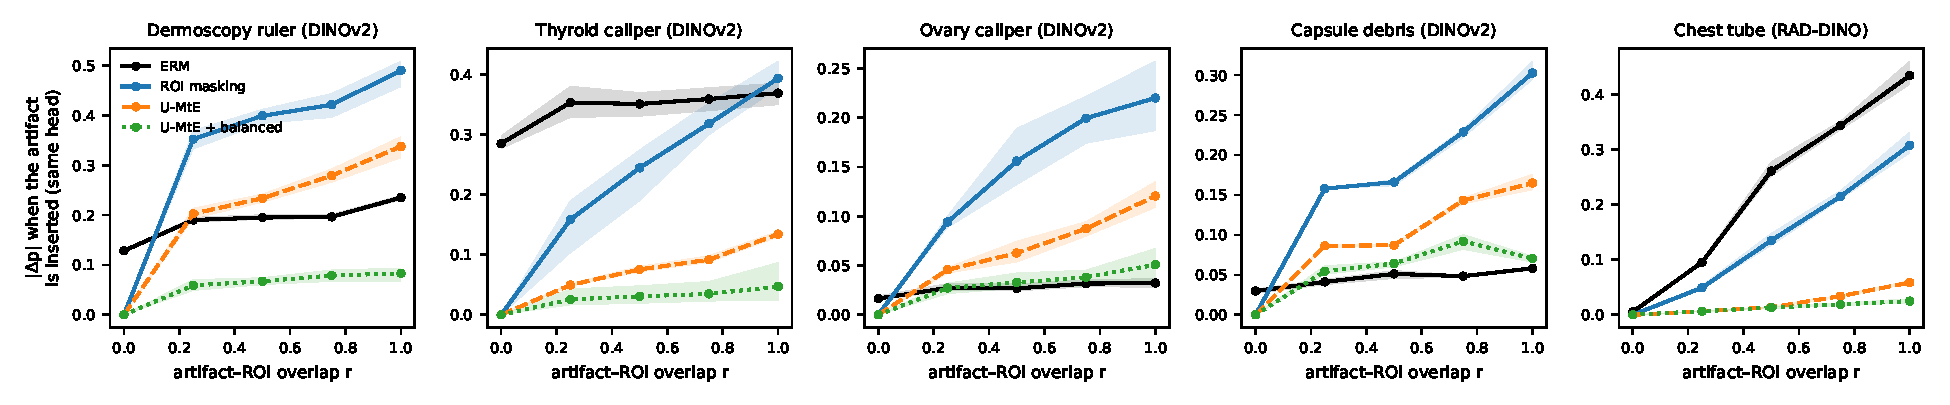
\includegraphics[width=\linewidth]{figures/mechanism.pdf}
\caption{Mechanism: same-head counterfactual sensitivity $|p(x{+}\text{artifact})-p(x)|$ versus the artifact's overlap
with the ROI in the five controlled sweeps (mean over seeds; band: range over seeds). Masking removes the out-of-ROI
artifact ($r=0$) but increasingly relies on an in-ROI one; erasure and balancing remove that reliance. Generated by
\texttt{scripts/analysis/mechanism\_figure.py}.}\label{fig:mechanism}\end{figure}

\paragraph{What the real-hair shortcut is made of}
Removing hair pixels at test time only closes 44--47\% of the ERM clean--reversed gap: most of what a frozen
encoder exploits in a real hair trap is not the hair pixels but what accompanies hair (hair-bearing images differ in
sex, age and body site). This bounds every pixel-level method, including oracle inpainting and U-MtE, and
explains why image-level-label methods, which remove everything correlated with the label, recover more.
